%!TEX root = ../../Main.tex
\graphicspath{{Chapters/Motormontering/}}
%-------------------------------------------------------------------------------

\chapter{Transport::recieve}

\lstset{language=C++}          % Set your language (you can change the language for each code-block optionally)

I teansport recieve skal vi modtage bufferen fra linklaget, samtidig med at vi skal transportere bufferen videre til applikationslaget. 
ifølge koden kører vi først en do, som kører så længe vores modtaget ack, er false. Denne ack, kommer fra checkChecksum, som validerer vores header, som består af 4 værdier. 
\begin{figure}[H]
\centering
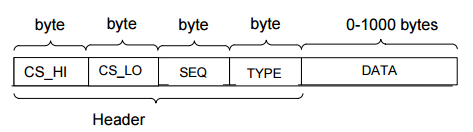
\includegraphics[width = 300 pt]{Img/header.PNG}
\caption{Header tansportlag}
\label{fig:konceptbillede}
\end{figure}

Til at starte med opretter vi først en lokal variable, som gemmer værdien fra link::recieve. 
Hvis Enable debuggeren er true, udskriver vi bufferen. Herefter opretter vi ack, som ifølge overstående blvier brugt som validering. Derfor sender vi også en sendAck(false), hvis vores modtaget ack er false. Vi laver også en errorhandling hvis vi modtager den samme pakke, vi sætter ack til false, da while løkken skal køre igen, men sender et true til sendAck(), da den derved får afvide vi gerne vil have den skal sende igen. 

Hvis/når ack'en bliver true, sender vi et true til sendAck(), dette gøres så den ved at den gerne må sende næste buffer. 
Herefter overskriver vi den gamle sekvens nummer med den nye. og til sidste ligger vi vores modtaget buffer, over i buf, som derved kan sendes videre til applikationslaget. 

\begin{lstlisting}[frame=single]  % Start your code-block

short Transport::receive(char buf[], short sizeApp)
{
    int currentSize = 0;
    bool ACK_;
    int i;

    do{
        currentSize = link->receive(buffer, sizeApp+ACKSIZE);

        ACK_ = checksum->checkChecksum (buffer, currentSize);

        if(ACK_ == false)
            sendAck(false);

        if(buffer[SEQNO] == old_seqNo)  
        //Registrere hvis vi modtager den samme pakke igen.
        {
            ACK_ = false;   //Koer loop igen
            sendAck(true);
        }



    }while(ACK_ == false);

    sendAck(true);

    old_seqNo = buffer[SEQNO];

    for(i = 0; i < sizeApp && i < (currentSize-ACKSIZE); i++)
    {
        buf[i] = buffer[i+ACKSIZE];
    }

    return i;

}

\end{lstlisting}


